% ! TeX program = lualatex

\documentclass{homework}
% \usepackage{lua-visual-debug}
\usepackage{graphicx}
\usepackage{amsmath, amssymb, amsfonts}
\usepackage{array}
\usepackage{mathtools}
\usepackage{ulem}
\usepackage{tikz}
\usepackage{xcolor}
\usepackage{graphicx}
\usetikzlibrary {positioning}
\usetikzlibrary {calc}

\usepackage{macros-common}


\newenvironment{redmatrix}
  {\left[\array{@{}ccccc@{}}}
  {\endarray\right]}
\newenvironment{ropmatrix}
  {\array{@{}c@{}}}
  {\endarray}
\newcommand\opone[2]{\xrightarrow{(#1)\times r_#2}}
\newcommand\optwo[3]{\xrightarrow{r_#1{}+{} #2r_#3}}
\def\opmult#1#2{\xrightarrow{E(#1;#2)}}
\def\opswap#1#2{\xrightarrow{E(#1,#2)}}
\def\opadd#1#2\to#3{\xrightarrow{E(#2,#3;#1)}}

\title{Midterm Homework}
\subject{MAS109(E,F) Introduction to Linear Algebra}
\studentid{20170058}
\name{Keonwoo Kim}
\date{\today}

\allowdisplaybreaks

\begin{document}
\maketitle

\solution{
(a)
\begin{alignat*}{5}
     &
    \begin{redmatrix}
        2&2&4&4&6\\
        3&3&6&4&7\\
        0&2&2&2&4\\
        1&2&3&3&5\\
        2&2&4&4&6\\
    \end{redmatrix}
     &
    \begin{ropmatrix}
        \opswap{2}{3}
    \end{ropmatrix}
     &
    \begin{redmatrix}
        2&2&4&4&6\\
        0&2&2&2&4\\
        3&3&6&4&7\\
        1&2&3&3&5\\
        2&2&4&4&6\\
    \end{redmatrix}
     &
    \begin{ropmatrix}
        \opmult{1}{1/2}
    \end{ropmatrix}
     &
    \begin{redmatrix}
        1&1&2&2&3\\
        0&2&2&2&4\\
        3&3&6&4&7\\
        1&2&3&3&5\\
        2&2&4&4&6\\
    \end{redmatrix}      \\
     &   &
    \begin{ropmatrix}
        \opadd{-3}{1}\to{3} \\
        \opadd{-1}{1}\to{4} \\
        \opadd{-2}{1}\to{5}
    \end{ropmatrix}
     &
    \begin{redmatrix}
        1&1&2&2&3\\
        0&2&2&2&4\\
        0&0&0&-2&-2\\
        0&1&1&1&2\\
        0&0&0&0&0\\
    \end{redmatrix}
     &
    \begin{ropmatrix}
        \opmult{2}{1/2}
    \end{ropmatrix}
     &
    \begin{redmatrix}
        1&1&2&2&3\\
        0&1&1&1&2\\
        0&0&0&-2&-2\\
        0&1&1&1&2\\
        0&0&0&0&0\\
    \end{redmatrix}      \\
     &   &
    \begin{ropmatrix}
        \opadd{-1}{2}\to{4}
    \end{ropmatrix}
     &
    \begin{redmatrix}
        1&1&2&2&3\\
        0&1&1&1&2\\
        0&0&0&-2&-2\\
        0&0&0&0&0\\
        0&0&0&0&0\\
    \end{redmatrix}
     &
    \begin{ropmatrix}
        \opmult{3}{-1/2}
    \end{ropmatrix}
     &
    \begin{redmatrix}
        1&1&2&2&3\\
        0&1&1&1&2\\
        0&0&0&1&1\\
        0&0&0&0&0\\
        0&0&0&0&0\\
    \end{redmatrix} = U \\
     &   &
    \begin{ropmatrix}
        \opadd{-2}{3}\to{1} \\
        \opadd{-1}{3}\to{2}
    \end{ropmatrix}
     &
    \begin{redmatrix}
        1&1&2&0&1\\
        0&1&1&0&1\\
        0&0&0&1&1\\
        0&0&0&0&0\\
        0&0&0&0&0\\
    \end{redmatrix}
     &
    \begin{ropmatrix}
        \opadd{-1}{2}\to{1}
    \end{ropmatrix}
     &
    \begin{redmatrix}
        1&0&1&0&0\\
        0&1&1&0&1\\
        0&0&0&1&1\\
        0&0&0&0&0\\
        0&0&0&0&0\\
    \end{redmatrix}
\end{alignat*}

\noindent (b) $PA=LU$ where
$$  P = E(2,3) =
    \begin{redmatrix}
        1&0&0&0&0\\
        0&0&1&0&0\\
        0&1&0&0&0\\
        0&0&0&1&0\\
        0&0&0&0&1\\
    \end{redmatrix}, \qquad U =
    \begin{redmatrix}
        1&1&2&2&3\\
        &1&1&1&2\\
        &&0&1&1\\
        &&&0&0\\
        &&&&0\\
    \end{redmatrix},$$
\begin{align*}
    L & = [E(3;-1/2)E(2,4;-1)E(2;1/2)E(1,5;-2)E(1,4;-1)E(1,3;-3)E(1;1/2)]^{-1}
    \\ &=
    \begin{redmatrix}
        2&&&&\\
        0&2\\
        3&0&-2\\
        1&1&0&1\\
        2&0&0&0&1
    \end{redmatrix}.
\end{align*}
(Empty spots are filled with zeroes.)

\noindent(c) Note that $B = \mathbf b_1 \mathbf v_1^T +\mathbf b_2 \mathbf v_2^T +\mathbf b_4 \mathbf v_3^T$, where
\[\begin{array}{lll}
        \mathbf b_1 = [1,0,0,0]^T ,  & \mathbf b_2 = [0,1,0,0]^T,   & \mathbf b_4 = [0,0,1,0]^T    \\
        \mathbf v_1 = [1,0,2,0,3]^T, & \mathbf v_2 = [0,1,4,0,5]^T, & \mathbf v_3 = [0,0,0,1,6]^T.
    \end{array}\]
Letting a composition of elementary row operations $E=E_n\cdots E_1$ be operated on $M$ to produce the RREF $B=EM$, we have $EM = E[\mathbf c_1,\dots,\mathbf c_5] = B = [\mathbf b_1,\dots,\mathbf b_5]$. Thus,
$$ M = E^{-1}B = E^{-1}\mathbf b_1 \mathbf v_1^T +E^{-1}\mathbf b_2 \mathbf v_2^T +E^{-1}\mathbf b_4 \mathbf v_3^T= \mathbf c_1 \mathbf v_1^T +\mathbf c_2 \mathbf v_2^T +\mathbf c_4 \mathbf v_3^T. $$
Hence, $\mathbf u_1 = \mathbf c_1$, $\mathbf u_2 = \mathbf c_2$, $\mathbf u_3 = \mathbf c_4$, and $\mathbf v_i$'s as above make the given equality true.
}

\solution{
    Since $A$ is of rank $k$, the RREF $R = EA$ ($E$: a product of elementary matrices) of $A$ has exactly $k$ nonzero rows. Then, as in the problem 1(c),
    $$ R \eqqcolon [\mathbf v_1,\cdots,\mathbf v_k,\mathbf 0\cdots,\mathbf 0]^T,\qquad R = \sum_{i=1}^k \mathbf e_i \mathbf v_i^T. $$
    Here, $\mathbf v_i$'s are linearly independent since they are the rows of the RREF $R$.
    Therefore, $A = E^{-1}R = \sum_{i=1}^k (E^{-1}\mathbf e_i) \mathbf v_i^T$. Note that the one-hot vectors $\mathbf e_i$ ($i=1,\dots,k$) are linearly independent, and the multiplication of $E^{-1}$, an invertible matrix, does not affect to the linear independence. Therefore, $\mathbf u_i \coloneqq E^{-1} \mathbf e_i$ ($i=1,\dots, k$) form a linearly independent set. This completes the proof.
}

\solution{
    \noindent(a) Suppose they are linearly independent. Then there are $a,b,c,d\in\RR$, where not all of them are zero, such that
    $$ ax e^x\cos x+bxe^x\sin x + ce^x\cos x + de^x\sin x= 0 $$
    for any $x\in \RR$. Equivalently,
    $$ ax \cos x+bx\sin x + c\cos x + d\sin x= 0 $$
    for any $x\in\RR$. Evaluating it at $x=0$, we get $c=0$. Evaluating it at $x = 2\pi$, we have $a\cdot 2\pi = 0$, that is, $a=0$. Then, $bx\sin x + d\sin x = 0$ for any $x\in\RR$. Dividing the both side by $\sin x$ assuming $\sin x$ is nonzero, we have $bx + d=0$, at least for two values of $x$. This implies $b=d=0$. This contradicts to the initial assumption.

    \noindent(b)
    \begin{align*}
        \frac{d}{dx}\,x e^x \cos x & = xe^x\cos x - xe^x\sin x + e^x\cos x, \\
        \frac{d}{dx}\,x e^x \sin x & = xe^x\sin x + xe^x\cos x + e^x\sin x, \\
        \frac{d}{dx}\,  e^x \cos x & = e^x\cos x - e^x\sin x,               \\
        \frac{d}{dx}\,  e^x \sin x & = e^x\sin x + e^x\cos x.
    \end{align*}
    Therefore,
    $$ [D]_{\mathcal B} = \begin{bmatrix}
            1  & 1 & 0  & 0 \\
            -1 & 1 & 0  & 0 \\
            1  & 0 & 1  & 1 \\
            0  & 1 & -1 & 1
        \end{bmatrix} .$$

    \noindent(c) The characteristic polynomial of $D$ is
    \begin{align*}
        p_{[D]_{\mathcal B}}(t) = t^4 - 4t^3 + 8t^2 - 8t + 4 = (t^2-2t+2)^2.
    \end{align*}
    So the eigenvalues are $1\pm i$. By a simple calculation,
    \begin{align*}
         & [D]_{\mathcal B}[\mathbf v]_{\mathcal B} = (1+i)[\mathbf v]_{\mathcal B} \implies [\mathbf v]_{\mathcal B} = c (0, 0, 1, i)^T,\text{\quad and} \\
         & [D]_{\mathcal B}[\mathbf v]_{\mathcal B} = (1-i)[\mathbf v]_{\mathcal B} \implies [\mathbf v]_{\mathcal B} = c (0, 0, i, 1)^T
    \end{align*}
    for an arbitrary $c\in\CC$.
    Therefore, the eigenvectors corresponding to $\lambda = 1+i$ is $ce^x(\cos x + i\sin x) = ce^{(1+i)x}$; and the eigenvectors corresponding to $\lambda = 1-i$ is $ce^x(\cos x - i\sin x) = ce^{(1-i)x}$, for $c\in\CC$.
}

\solution{
    Let me solve (b) first and then (a).

    \noindent(b) Take $\mathbf v_1 = \frac 1 {\sqrt 3} (1,1,1)
        ^T$, and a (unit) vector $\mathbf v_2 = \frac 1 {\sqrt 2} (1,0,-1)^T$ in the orthogonal complement of $\mathbf v_1$. Finally, let $\mathbf v_3 =\mathbf v_1 \times \mathbf v_2 = \frac 1{\sqrt6}(-1, 2, -1)^T$. Then, $T$ becomes a rotation following the right-hand direction with respect to the basis $\mathcal B = \{\mathbf v_1,\mathbf v_2,\mathbf v_3\}$, that is, the direction of other fingers when the thumb is pointing the vector $(1,1,1)^T$. Thus, $T$ is a CCW rotation on a plane orthogonal to $\mathbf v_1$, so that
    $$ [T]_{\mathcal B} = \begin{bmatrix}
            1 & 0              & 0               \\
            0 & \cos(30^\circ) & -\sin(30^\circ) \\
            0 & \sin(30^\circ) & \cos(30^\circ)  \\
        \end{bmatrix} = \begin{bmatrix}
            1 & 0           & 0           \\
            0 & \sqrt 3 / 2 & -1/2        \\
            0 & 1/2         & \sqrt 3 / 2 \\
        \end{bmatrix}. $$

    \noindent(a) Letting
    $$ P = \begin{bmatrix}
            \frac 1{\sqrt 3} & \frac 1{\sqrt 2}  & -\frac 1{\sqrt 6} \\
            \frac 1{\sqrt 3} & 0                 & \frac 2{\sqrt 6}  \\
            \frac 1{\sqrt 3} & -\frac 1{\sqrt 2} & -\frac 1{\sqrt 6} \\
        \end{bmatrix}, $$
    we have $[T]_{\mathcal E} = P [T]_{\mathcal B} P^{-1}$ where $\mathcal E$ is the standard basis of $\RR^3$. By a simple calculation, using $P^{-1} = P^T$, we get
    $$ [T]_{\mathcal E} = \frac 1 3 \begin{bmatrix}
            1+\sqrt 3 & 1-\sqrt 3 & 1         \\
            1         & 1+\sqrt 3 & 1-\sqrt 3 \\
            1-\sqrt 3 & 1         & 1+\sqrt 3
        \end{bmatrix}. $$
}

\solution{
\noindent(a) Note $W = \operatorname{col}(A)$ where $A = [\mathbf u_1, \mathbf u_2]$, and
\begin{align*}
    [T]_{\mathcal E} = A(A^TA)^{-1}A^T.
\end{align*}
\noindent(b) Taking an orthogonal basis $\mathcal B$ extending $\{\mathbf u_1,\mathbf u_2\}$ which exists due to, say, Gram--Schmidt orthogonalization, we have
\begin{align*}
    [T]_{\mathcal B} = \begin{bmatrix}
        1      & 0      & 0      & \cdots & 0      \\
        0      & 1      & 0      & \cdots & 0      \\
        0      & 0      & 0      & \cdots & 0      \\
        \vdots & \vdots & \vdots & \ddots & \vdots \\
        0      & 0      & 0      & \cdots & 0
    \end{bmatrix} = \begin{bmatrix}
        I_2 & O_{2\times (n-2)} \\ O_{(n-2)\times 2} & O_{(n-2)\times (n-2)}
    \end{bmatrix}.
\end{align*}
}

\solution{
(a) The characteristic polynomial of $A$ is
\begin{align*}
    \det(tI - A) = t^4 - 16t^3 - 20t^2 = t^2(t^2-16t-20).
\end{align*}
Thus, the eigenvalues are $\lambda_1 = 8 + 2\sqrt{21}$, $\lambda_2 = 8 -2\sqrt{21}$, and $\lambda_3=\lambda_4=0$. Corresponding eigenvectors are:
\begin{itemize}
    \item $\mathbf v_1= ({13+3 \sqrt{21},18+4 \sqrt{21},23+5 \sqrt{21},28+6 \sqrt{21}})^T$,
    \item $\mathbf v_2= ({-13+3 \sqrt{21},-18+4 \sqrt{21},-23+5 \sqrt{21},-28+6 \sqrt{21}})^T$,
    \item $\mathbf v_3= (2,-3, 0, 1)^T$,
    \item $\mathbf v_4= (1, 2,-7, 4)^T$.
\end{itemize}
Normalizing them, we obtain
\begin{itemize}
    \item $\mathbf u_1= \frac{1}{2 \sqrt{903+197 \sqrt{21}}}\mathbf v_1$,
    \item $\mathbf u_2=  \frac{1}{2 \sqrt{903-197 \sqrt{21}}}\mathbf v_2$,
    \item $\mathbf u_3= \frac{1}{\sqrt {14}} \mathbf v_3$,
    \item $\mathbf u_4= \frac{1}{\sqrt {70}} \mathbf v_4$.
\end{itemize}
Let $P = [\mathbf u_1,\cdots,\mathbf u_4]$. Then the orthogonal diagonalization of $A$ is
$$ P^T A P = \operatorname{diag}(\lambda_1,\lambda_2,\lambda_3,\lambda_4) = \operatorname{diag}(8+2\sqrt{21},8-2\sqrt{21},0,0).$$

\noindent(b) The spectral decomposition of $A$ is
\begin{align*}
    A & = (8+2\sqrt{21})\mathbf u_1 \mathbf u_1^T +  (8-2\sqrt{21})\mathbf u_2 \mathbf u_2^T
    \\&\paren{= \frac{8+2\sqrt{21}}{4{(903+197 \sqrt{21})}} \mathbf v_1\mathbf v_1^T + \frac{8-2\sqrt{21}}{4({903-197 \sqrt{21}})} \mathbf v_2\mathbf v_2^T}
\end{align*}
where $\mathbf u_1,\mathbf u_2,\mathbf v_1,\mathbf v_2$ are as in (a).

\noindent(c) Singular values of $A^TA=A^2$ are $\lambda_i^2$ ($i=1,2$), which are $(8\pm 2\sqrt{21})^2.$

\noindent(d)
\begin{align*}
    e^A & = \sum_{k\ge 0} \frac 1{k!} A^k
    \\ &= \sum_{k\ge 0} \frac 1{k!} (\lambda_1^k \mathbf u_1\mathbf u_1^T + \lambda_2^k \mathbf u_2\mathbf u_2^T)
    \\ &= \sum_{k\ge 0} \frac 1{k!} ((8+ 2\sqrt{21})^k \mathbf u_1\mathbf u_1^T + (8- 2\sqrt{21})^k \mathbf u_2\mathbf u_2^T)
\end{align*}
where $\mathbf u_1,\mathbf u_2$ are as in (a).

\noindent(e) Let $\mathbf w_1 = (1,2,3,4)^T$ and $\mathbf w_2 = (2,3,4,5)^T$, then an orthogonal basis $\{\mathbf q_1,\mathbf q_2\}$ for $\operatorname{span}(\mathbf w_1,\mathbf w_2)$ is given by
$$ \mathbf v_1 = \mathbf w_1,\qquad \mathbf q_1 = \frac 1{\sqrt{30}}(1,2,3,4)^T, $$
and
$$ \mathbf v_2 = \mathbf w_2 - \operatorname{proj}_{\mathbf w_1}\mathbf w_2 = (2,3,4,5) - \frac{4}{3}(1,2,3,4)^T = \frac 1 3(2,1,0,-1)^T $$
$$ \mathbf q_2 = \frac 1{\sqrt{6}}(2,1,0,-1)^T. $$
Extend $\set{\mathbf q_1,\mathbf q_2}$ into an orthonormal basis of $\RR^4$. Letting $\mathbf w_3 = (1,0,0,0)^T$, we have
$$ \mathbf v_3 = \mathbf w_3 - (\mathbf w_3 \cdot \mathbf q_1)\mathbf q_1 - (\mathbf w_3 \cdot \mathbf q_2)\mathbf q_2 = \frac 1 {10}(3,-4,-1,2)^T, $$
$$ \mathbf q_3 = \frac 1 {\sqrt{30}}(3,-4,-1,2)^T. $$
Letting $\mathbf w_4 = (0,1,0,0)^T$, we have
$$ \mathbf v_4 = \mathbf w_4 - (\mathbf w_4 \cdot \mathbf q_1)\mathbf q_1 - (\mathbf w_4 \cdot \mathbf q_2)\mathbf q_2 - (\mathbf w_4 \cdot \mathbf q_3)\mathbf q_3 = \frac 1 {6}(0,1,-2,1)^T, $$
$$ \mathbf q_4 = \frac 1 {\sqrt{6}}(0,1,-2,1)^T. $$
Thus, $Q = [\mathbf q_1,\cdots,\mathbf q_4]$ is an orthogonal matrix. With $A = [\mathbf a_1,\cdots,\mathbf a_4]$,
$$ R = \begin{bmatrix}
        \mathbf a_1\cdot \mathbf q_1 & \mathbf a_2\cdot \mathbf q_1 & \mathbf a_3\cdot\mathbf q_1 & \mathbf a_4\cdot \mathbf q_1 \\
        0                            & \mathbf a_2\cdot \mathbf q_2 & \mathbf a_3\cdot\mathbf q_2 & \mathbf a_4\cdot \mathbf q_2 \\
        0                            & 0                            & 0                           & 0                            \\
        0                            & 0                            & 0                           & 0
    \end{bmatrix} = \begin{bmatrix}
        \sqrt{30} & \frac 43\sqrt{3} & \frac 53\sqrt{3} & 2\sqrt3 \\
        0         & \frac13 \sqrt 6  & \frac23 \sqrt 6  & \sqrt 6 \\
        0         & 0                & 0                & 0       \\
        0         & 0                & 0                & 0
    \end{bmatrix} $$
where $A=QR$.

\noindent(f) The SVD of $A$ is given by $A=U\Sigma V^T$, where $A^TA$ has eigenvalues $\sigma_1^2 = (8+ 2\sqrt{21})^2$, $\sigma_2^2 = (8-2\sqrt{21})^2$ and $\lambda_3=\lambda_4=0$ (with multiplicity 2), and the (unit) eigenvectors
$$ V = [\mathbf v_1,\cdots,\mathbf v_4] = \begin{bmatrix}
        -0.3147 & 0.7752  & 0.3041  & -0.4556 \\
        -0.4275 & 0.3424  & -0.0659 & 0.8341  \\
        -0.5402 & -0.0903 & -0.7805 & -0.3015 \\
        -0.6530 & -0.5231 & 0.5423  & -0.0770
    \end{bmatrix} $$
(where $\mathbf v_i$ corresponds to $\sigma_i^2$.) And $\mathbf u_i = A\mathbf v_i/\sigma_i$ for $i=1,2$, yielding
\begin{align*}
    \mathbf u_1 & = (-0.3147, -0.4275, -0.5402, -0.6530)^T, \\\mathbf u_2 &= (-0.7752,-0.3424,0.0903,0.5231)^T.
\end{align*}
Extending $\{\mathbf u_1, \mathbf u_2\}$ to an orthogonal basis of $\RR^4$, we have
\begin{align*}
    U = [\mathbf u_1,\dots,\mathbf u_4] = \begin{bmatrix}
        -0.3147 & -0.7752 & 0.5442  & 0.0619  \\
        -0.4275 & -0.3424 & -0.7718 & 0.3231  \\
        -0.5402 & 0.0903  & -0.0891 & -0.8319 \\
        -0.6530 & 0.5231  & 0.3167  & 0.4469
    \end{bmatrix}.
\end{align*}
With $\Sigma = \operatorname{diag}(8+ 2\sqrt{21}, 8- 2\sqrt{21},0,0)$, we have $A = U\Sigma V^T$. Then, the following is the polar decomposition of $A$: $A=QS$ where
\begin{align*}
    Q & = UV^T = \begin{bmatrix}
        -0.3646 & -0.1152 & -0.2034 & 0.9014 \\
        -0.5128 & 0.3858  & 0.7668  & 0.0149 \\
        0.5919  & -0.4261 & 0.6040  & 0.3213 \\
        0.5037  & 0.8101  & -0.0764 & 0.2900
    \end{bmatrix},        \\
    S & = V\Sigma V^T = \begin{bmatrix}
        2.4004 & 2.6186 & 2.8368 & 3.0551 \\
        2.6186 & 3.2733 & 3.9279 & 4.5826 \\
        2.8368 & 3.9279 & 5.0190 & 6.1101 \\
        3.0551 & 4.5826 & 6.1101 & 7.6376
    \end{bmatrix}.
\end{align*}
}

\solution{
    \noindent(a) The characteristic polynomial of $A$ is
    \begin{align*}
        \det(tI - A) & = \det \begin{bmatrix}
            t-1 & -1 \\ -1 & t-1
        \end{bmatrix} \cdot \det \begin{bmatrix}
            t-2 & -2 & 0 \\ 0 & t-2 & -1 \\ 0&0&t-2
        \end{bmatrix} \cdot \det \begin{bmatrix}
            t & 0 \\ -1 & t
        \end{bmatrix} \\
                     & = [(t-1)^2-1](t-2)^3 t^2 = t^3 (t-2)^4.
    \end{align*}

    \noindent(b) Eigenvalues are $0$ and $2$. Eigenvectors corresponding to 0 are
    $$ (\uline{-1,1},0,0,0,0,0)^T,\quad (0,0,0,0,0,\uline{0,1})^T, $$
    and eigenvectors corresponding to 2 are
    $$ (\uline{1,1},0,0,0,0,0)^T,\quad (0,0,\uline{1,0,0},0,0)^T. $$

    \noindent(c) Algebraic multiplicities of eigenvalues 0 and 2 are \uline{3 and 4}, respectively. Geometric multiplicities of both eigenvalues are \uline{2}.

    \noindent(d) The minimal polynomial of $A$ has the factor $t$ and $t-2$. Since $A(A-2I),\ A(A-2I)^2,\ A(A-2I)^3,\ A^2(A-2I),\ A^2(A-2I)^2$ are nonzero and $A^2(A-2I)^3 = O_{7\times 7}$, the minimal polynomial of $A$ is $m_A(t) = t^2 (t-2)^3.$
}

\solution{
    \noindent Let $X = \begin{bmatrix}
            a & b \\c&d
        \end{bmatrix}$. Then
    $$T(X) = \begin{bmatrix}
            -3 b + 2 c      & -2 a - 3 b + 2 d \\
            3 a + 3 c - 3 d & 3 b - 2 c
        \end{bmatrix}. $$

    \noindent(a) The kernel of $T$ is
    \begin{align*}
        \ker T = \set{\begin{bmatrix}
                a & b \\ c & d
            \end{bmatrix} : 3b = 2c,\, d = a+c } = \set{ \begin{bmatrix}
                a & 2c/3 \\ c & a+c
            \end{bmatrix}:a,\,c\in\RR^4 }.
    \end{align*}

    \noindent(b) With the standard basis $\mathcal E = \{\mathbf e_1,\dots,\mathbf e_4\}$ where
    \[ \mathbf e_1 = \begin{bmatrix}1&0\\0&0\end{bmatrix},\ \mathbf e_2 = \begin{bmatrix}0&1\\0&0\end{bmatrix}, \ \mathbf e_3 = \begin{bmatrix}0&0\\1&0\end{bmatrix},\ \mathbf e_4 = \begin{bmatrix}0&0\\0&1\end{bmatrix}, \]
    we have
    \begin{align*}
        T\mathbf e_1 & = -2 \mathbf e_2 + 3\mathbf e_3,                \\
        T\mathbf e_2 & = -3 \mathbf e_1 - 3\mathbf e_2 + 3\mathbf e_4, \\
        T\mathbf e_3 & = 2 \mathbf e_1 + 3\mathbf e_3 - 2\mathbf e_4,  \\
        T\mathbf e_4 & = 2 \mathbf e_2 - 3\mathbf e_3,                 \\
    \end{align*}
    so that $$[T]_{\mathcal E} = \begin{bmatrix}
            0  & -3 & 2  & 0  \\
            -2 & -3 & 0  & 2  \\
            3  & 0  & 3  & -3 \\
            0  & 3  & -2 & 0
        \end{bmatrix}.$$ Thus, the characteristic polynomial of $T$ is the same with $\det(tI - [T]_{\mathcal E}) = t^4 - 33t^2.$
}

\solution{
I will show the following: (the arrows mean the implications)



\definecolor {processblue}{cmyk}{0.96,0,0,0}
\begin {center}
\hspace*{-1.2cm}\begin {tikzpicture}[-latex ,auto ,node distance =2cm and 2cm ,on grid ,
    semithick ,
    state/.style ={ rectangle, draw, minimum width =8mm, minimum height=8mm}]
\node[state] (A) { (a) };
\node[state] (B) [right=of A] { (b) };
\node[state] (C) [right=of B] { (c) };
\node[state] (D) [right=of C] { (d) };
\node[state] (E) [right=of D] { (e) };
\node[state] (Q) [below=of E] { (q) };
\node[state] (Q') [below right=of Q] { (q') };
\node[state] (G) [below=of B] { (g) };
\node[state] (H) [right=of G] { (h) };
\node[state] (J) [right=of E] { (j) };
\node[state] (F) [right=of J] { (f) };
\node[state] (I) [right=of F] { (i) };
\node[state] (N) [below=of Q'] { (n) };
\node[state] (K) [right=of N] { (k) };
\node[state] (L) [right=of K] { (l) };
\node[state] (M) [left=of N] { (m) };
\node (MK) [below=of N] {};
\node (NL) [below=of K] {};
\node[state] (O) [below=of MK] { (o) };
\node[state] (P) [below=of NL] { (p) };
\node[state] (R) [above right=of Q'] { (r) };
\node[state] (R') [below right=of R] { (r') };

\node[state] (S) [below=of H] { (s) };
\node[state] (T) [below=of G] { (t) };

\draw[->] (A) -- (B);
\draw[->] (B) -- (C);
\draw[->] (C) -- (D);
\draw[->] (D) -- (E);
\draw[<->] (D) -- (H);
\draw[<->] (G) -- (H);

\draw[<->] (E) -- (J);
\draw[<->] (F) -- (I);
\draw[<->] (E) -- (Q);
\draw[<->] (D) -- (R);

\path[<->] (F) edge [bend left =-25] (D);
\path[->] (O) edge [bend left =30] (M);
\path[->] (P) edge [bend left =30] (N);


\draw[<->] (Q) -- (R);
\draw[<->] (Q) -- (Q');
\draw[<->] (Q') -- (R');
\draw[<->] (Q) -- (M);
\draw[<->] (Q') -- (N);
\draw[<->] (R) -- (K);
\draw[<->] (R') -- (L);

\draw[<->] (Q) -- (S);
\draw[<->] (Q) -- (T);

\draw[->] (Q) -- (A);

\draw[-] (M) -- ($(MK) + ( 0.01,-0.01)$);
\draw[-] (K) -- ($(MK) + (-0.01,-0.01)$);
\draw[->] ($(MK) + (0,0.01)$) -- (O);

\draw[-] (N) -- ($(NL) + ( 0.01,-0.01)$);
\draw[-] (L) -- ($(NL) + (-0.01,-0.01)$);
\draw[->] ($(NL) + (0,0.01)$) -- (P);

\end{tikzpicture}
\end{center}
where (q') $\operatorname{rank}(A^T)=n$ and (r') $\operatorname{nullity}(A^T)=0$.

\def\impl{$\implies$}
\def\eq{\,$\Longleftrightarrow$\,}
\noindent(a)\impl(b): Since $A$ is row-equivalent to $I_n$, there is matrix $E=E_n\cdots E_1$ which is a product of elementary matrices such that $EA = I_n$. Then $A = E_1^{-1}\cdots E_n^{-1}$, where each $E_i^{-1}$ is again an elementary matrix. Thus, $A$ is expressible as a product of elementary matrices.

\noindent(b)\impl(c): If $A=E_n\cdots E_1$, $A^{-1} = E_1^{-1}\cdots E_n^{-1}$.

\noindent(c)\impl(d): $A\mathbf x = \mathbf 0$ implies $\mathbf x = A^{-1}A\mathbf x = A\mathbf 0 = \mathbf 0$.

\noindent(d)\impl(e): There is a solution $\mathbf b = A^{-1}\mathbf x$ to the equation $A\mathbf x = \mathbf b$.

\noindent(e)\eq(j): By definition.

\noindent(d)\eq(h): $\lambda=0$ is an eigenvalue of $A$ iff there is a nonzero vector $\mathbf x$ such that $A\mathbf x = 0\mathbf x = \mathbf 0$. The contrapositive of this statement is exactly (d)\eq(h).

\noindent(h)\eq(g): $\lambda=0$ is an eigenvalue of $A$ iff $\det(tI - A)|_{t=0} = (-1)^n\det(A) =0$ iff $\det(A) = 0$. The contrapositive of this statement is exactly (h)\eq(g).

\noindent(e)\eq(q): (e) iff $T_A(\RR^n) = \RR^n$ iff $T_A(\RR^n)$, which is a subspace of $\RR^n$, has the dimension $n$ iff $\operatorname{rank}(A)=n$. 

\noindent(d)\eq(f): $(\Longleftarrow)$ is clear. $(\Longrightarrow)$ If $A\mathbf x_1 = \mathbf b = A \mathbf x_2$, then $A(\mathbf x_1-\mathbf x_2)=\mathbf 0$ so that $\mathbf x_1-\mathbf x_2$, a solution of $A\mathbf x = \mathbf 0$, should be $\mathbf 0$.

\noindent(d)\eq(r): By definition.

\noindent(f)\eq(i): By definition.

\noindent(q)\impl(a): Since the rank of $A$ and the rref of $A$ are the same, the rref of $A$ has rank $n$. Since $I_n$ is the only possible candidate of rref having the rank $n$, the rref of $A$ should be $I_n$.

\noindent(q)\eq(r): The rank--nullity theorem implies this.

\noindent(q)\eq(q'): $\operatorname{rank}(A) = \operatorname{rank}(A^T)$.

\noindent(q')\eq(r'): The rank--nullity theorem implies this.

\noindent(q)\eq(r): The rank--nullity theorem implies this.

\noindent(q)\impl(m): The columns of $A$ span the subspace of the dimension $n$ in $\RR^n$, which is $\RR^n$.

\noindent(q')\impl(n): The columns of $A^T$, i.e. the (transposes of) rows of $A$, span the subspace of the dimension $n$ in $\RR^n$, which is $\RR^n$.

\noindent(q)\impl(k): Suppose the contrary. Then the columns, $A\mathbf e_i$, of $A$ has a linear dependency for some $a_i\in\RR$ which are not simultaneously zero:
$$ \sum_{i=1}^n a_i A\mathbf e_i = A \sum_{i=1}^n a_i \mathbf e_i = \mathbf 0. $$
This implies $\mathbf 0\ne  \sum_{i=1}^n a_i \mathbf e_i\in \operatorname{null}(T_A)$, which leads to a contradiction that $\operatorname{nullity}(A)>0$.

\noindent(r')\impl(l): The analogous argument of the above works.

\noindent(m)\,$\land$\,(k)\impl(o): By definition.

\noindent(n)\,$\land$\,(l)\impl(p): By definition.

\noindent(o)\impl(m): By definition.

\noindent(p)\impl(n): By definition. (The columns of $A^T$ is the transposes of the rows of $A$.)

\noindent(q)\eq(s): $A$ has $n$ singular values iff $A^TA$ does not have $\sigma^2=0$ as an eigenvalue, which is equivalent, by (h)\eq(d)\eq(r)\eq(q), to that $\operatorname{rank}(A^TA) = n$. Therefore, (s)\eq $\operatorname{rank}(A^TA)=n$. Since $\operatorname{rank}(A^TA) = \operatorname{rank}(A)$, we have (q)\eq(s).

\noindent(q)\eq(t): $A$ is of rank $<n$ iff there are vectors $\mathbf v_1,\dots,\mathbf v_{n-1}\in\RR^n$ such that for the $i$-th column $A_i$ of $A$,
$$ A_i = \sum_{j=1}^{n-1} c_{ij}\mathbf v_j $$
for some $c_{ij}$'s. That is,
$$ A = \sum_{j=1}^{n-1} [c_{1j},\cdots, c_{nj}]\mathbf v_j. $$
for some $c_{ij}$'s. This is equivalent to that $A$ is a sum of $<n$ rank-one matrices $[c_{1j},\cdots,c_{nj}]\mathbf v_j$ ($j=1,\dots,n-1$).
}

\solution{
\noindent(a) When $n=2$,
\begin{align*}
    & A = \begin{bmatrix}
        1&0\\1&1
    \end{bmatrix}, \quad A^TA = \begin{bmatrix}
        2&1\\1&1
    \end{bmatrix},\quad p_{A^TA}(t) = \det(tI-A^TA) = t^2-3t+1,\\
    &\text{singular values: }\sqrt{\frac{3\pm\sqrt 5}{2}} = \frac{ \sqrt 5 \pm 1}2\approx 0.6180,\ 1.6180.
\end{align*}
When $n=3$,
\begin{align*}
    & A = \begin{bmatrix}
        1&0&0\\1&1&0\\1&1&1
    \end{bmatrix}, \quad A^TA = \begin{bmatrix}
        3&2&1\\2&2&1\\1&1&1
    \end{bmatrix},\quad p_{A^TA}(t) = t^3 - 6t^2 + 5t - 1,\\
    &\text{singular values: }0.554958,\ 0.801938,\ 2.246980.
\end{align*}
When $n=4$,
\begin{align*}
    & A = \begin{bmatrix}
        1&0&0&0\\1&1&0&0\\1&1&1&0\\1&1&1&1
    \end{bmatrix}, \quad A^TA = \begin{bmatrix}
        4&3&2&1\\3&3&2&1\\2&2&2&1\\1&1&1&1
    \end{bmatrix},\\
    & p_{A^TA}(t) = t^4 - 10t^3 + 15t^2 - 7t + 1 = (t-1)(t^3 - 9t^2 + 6t - 1),\\
    &\text{singular values: }
    0.532089,\ 
    0.652704,\ 
    1,\ 
    2.879385.
\end{align*}

\noindent(b)
\begin{itemize}
    
\item $n=10$:
$(6.6907, 2.2470, 1.3686, 1.0000, 0.8019, 0.6821, 0.6052, 0.5550, 0.5232, 0.5056)$

\item $n=20$:
$(13.0539, 4.3598, 2.6262, 1.8869, 1.4792, 1.2223, 1.0466, 0.9198, 0.8248, 0.7515, \dots)$

\item $n=30$:
$(19.4190, 6.4787, 3.8941, 2.7889, 2.1769, 1.7890, 1.5219, 1.3272, 1.1795, 1.0639, \dots)$

\item $n=40$:
$(25.7847, 8.5992, 5.1647, 3.6946, 2.8794, 2.3618, 2.0045, 1.7434, 1.5445, 1.3882, \dots)$

\item $n=50$:
$(32.1506, 10.7203, 6.4363, 4.6018, 3.5838, 2.9370, 2.4900, 2.1629, 1.9133, 1.7169, \dots)$

\item $n=60$:
$(38.5166, 12.8417, 7.7085, 5.5098, 4.2893, 3.5133, 2.9768, 2.5840, 2.2841, 2.0478, \dots)$

\item $n=70$:
$(44.8826, 14.9634, 8.9810, 6.4182, 4.9952, 4.0904, 3.4645, 3.0061, 2.6559, 2.3799, \dots)$

\item $n=80$:
$(51.2487, 17.0851, 10.2536, 7.3268, 5.7015, 4.6679, 3.9527, 3.4288, 3.0284, 2.7128, \dots)$

\item $n=90$:
$(57.6148, 19.2069, 11.5264, 8.2356, 6.4081, 5.2456, 4.4413, 3.8518, 3.4014, 3.0461, \dots)$

\item $n=100$:
$(63.9809, 21.3287, 12.7993, 9.1446, 7.1148, 5.8236, 4.9300, 4.2751, 3.7746, 3.3798, \dots)$
\end{itemize}


\newpage
\noindent(c)
\begin{figure}[ht]
    \centering
    \hspace*{-2cm}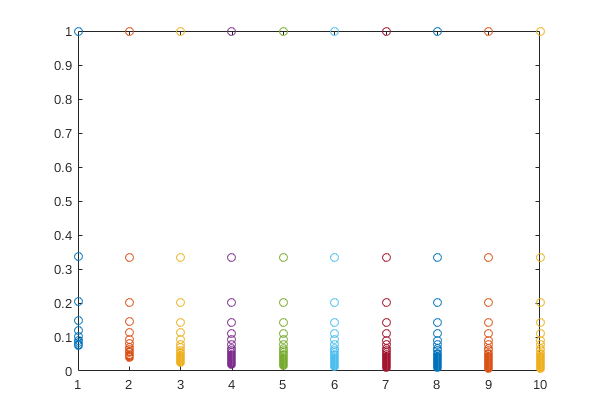
\includegraphics{midterm10c.png}    \caption{Figure for \#10 (c)}
\end{figure}

\noindent(d) Using the SVD $A = \sigma_1 \mathbf u_1^T \mathbf v_1^T + \cdots$ of $A$, the closest rank-one matrix to $A$ is 
\begin{align*}
    &\sigma_1 \mathbf u_1^T \mathbf v_1^T = \\&\begin{bmatrix}
    8.4793  &  8.2898  &  7.9152  &  7.3638  &  6.6479  &  5.7835  &  4.7899  &  3.6893  &  2.5063  &  1.2673 \\
    8.2898  &  8.1047  &  7.7384  &  7.1993  &  6.4994  &  5.6543  &  4.6829  &  3.6069  &  2.4503  &  1.2390 \\
    7.9152  &  7.7384  &  7.3888  &  6.8740  &  6.2057  &  5.3988  &  4.4713  &  3.4439  &  2.3396  &  1.1830 \\
    7.3638  &  7.1993  &  6.8740  &  6.3952  &  5.7734  &  5.0227  &  4.1598  &  3.2040  &  2.1766  &  1.1006 \\
    6.6479  &  6.4994  &  6.2057  &  5.7734  &  5.2121  &  4.5344  &  3.7554  &  2.8925  &  1.9650  &  0.9936 \\
    5.7835  &  5.6543  &  5.3988  &  5.0227  &  4.5344  &  3.9448  &  3.2671  &  2.5164  &  1.7095  &  0.8644 \\
    4.7899  &  4.6829  &  4.4713  &  4.1598  &  3.7554  &  3.2671  &  2.7058  &  2.0841  &  1.4158  &  0.7159 \\
    3.6893  &  3.6069  &  3.4439  &  3.2040  &  2.8925  &  2.5164  &  2.0841  &  1.6052  &  1.0905  &  0.5514 \\
    2.5063  &  2.4503  &  2.3396  &  2.1766  &  1.9650  &  1.7095  &  1.4158  &  1.0905  &  0.7408  &  0.3746 \\
    1.2673  &  1.2390  &  1.1830  &  1.1006  &  0.9936  &  0.8644  &  0.7159  &  0.5514  &  0.3746  &  0.1894 
    \end{bmatrix}.
\end{align*}

\noindent(d) Using the SVD $A = \sigma_1 \mathbf u_1^T \mathbf v_1^T + \sigma_2 \mathbf u_2^T \mathbf v_2^T + \cdots$ of $A$, the closest rank-two matrix to $A$ is 
\begin{align*}
    &\sigma_1 \mathbf u_1^T \mathbf v_1^T + \sigma_2 \mathbf u_2^T \mathbf v_2^T = \\&\begin{bmatrix}
        9.3933  &  9.0229  &  8.3220  &  7.3638  &  6.2411  &  5.0505  &  3.8758  &  2.7752  &  1.7733  &  0.8605 \\
        9.0229  &  8.6925  &  8.0647  &  7.1993  &  6.1732  &  5.0665  &  3.9499  &  2.8739  &  1.8625  &  0.9128 \\
        8.3220  &  8.0647  &  7.5698  &  6.8740  &  6.0247  &  5.0726  &  4.0645  &  3.0371  &  2.0134  &  1.0020 \\
        7.3638  &  7.1993  &  6.8740  &  6.3952  &  5.7734  &  5.0227  &  4.1598  &  3.2040  &  2.1766  &  1.1006 \\
        6.2411  &  6.1732  &  6.0247  &  5.7734  &  5.3932  &  4.8607  &  4.1622  &  3.2993  &  2.2912  &  1.1746 \\
        5.0505  &  5.0665  &  5.0726  &  5.0227  &  4.8607  &  4.5327  &  4.0001  &  3.2494  &  2.2974  &  1.1906 \\
        3.8758  &  3.9499  &  4.0645  &  4.1598  &  4.1622  &  4.0001  &  3.6199  &  2.9982  &  2.1488  &  1.1227 \\
        2.7752  &  2.8739  &  3.0371  &  3.2040  &  3.2993  &  3.2494  &  2.9982  &  2.5193  &  1.8235  &  0.9582 \\
        1.7733  &  1.8625  &  2.0134  &  2.1766  &  2.2912  &  2.2974  &  2.1488  &  1.8235  &  1.3287  &  0.7008 \\
        0.8605  &  0.9128  &  1.0020  &  1.1006  &  1.1746  &  1.1906  &  1.1227  &  0.9582  &  0.7008  &  0.3705 
    \end{bmatrix}.
\end{align*}

}

\end{document}
